\chapter[SCP-180 身份窃取帽]{
    SCP-180 Identity Thieving Hat\\
    SCP-180 身份窃取帽
}

\label{chap:SCP-180}

\begin{figure}[H]
    \centering
    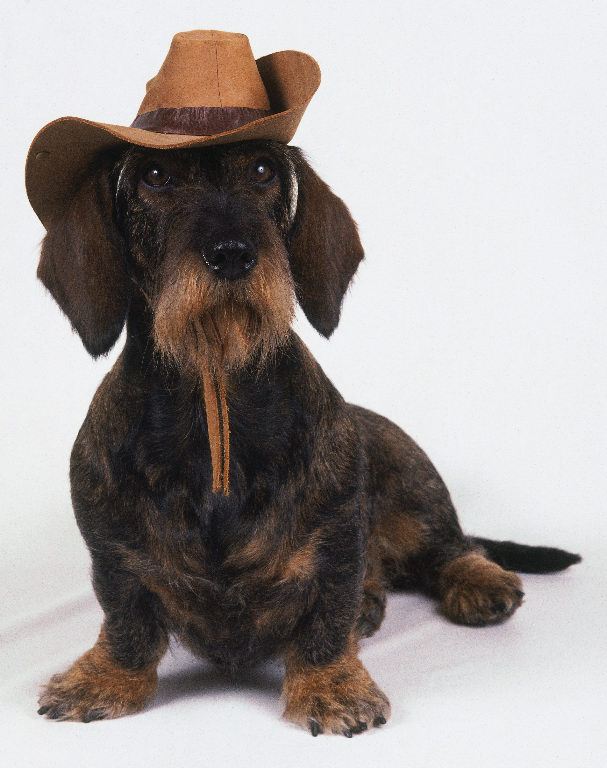
\includegraphics[width=0.5\linewidth]{images/SCP-180.jpg}
    \caption*{特工{[}删除]在照相机前摆好姿势。尽管他的外貌看上去是这样,他实际上是黑发蓝眼的33岁男人。SCP-180的原主是一只硬毛斑纹达克斯猎狗。}
\end{figure}

\bb{项目编号:}SCP-180

\bb{项目等级:}Euclid

\bb{特殊收容措施:}出于安全考虑,在圣物研究收容76处严格限制一切头饰(包括发夹和蝴蝶结)的佩戴。违反此规则者须接受身体搜查,在76处之内的行动,以及DNA鉴别测试。

SCP-180不能离开研究实验室。SCP-180当前外观须每日报告安保部门。一旦有人员在本部门中偶遇不认识却穿着或表现得如同是属于部门一般(他们的身份可能被窃取)的人,都应当立即通知安保部门。

\bb{描述:}SCP-180呈一顶帽子或者其他形式的头饰、发饰状。将SCP-180放在头上的个体身份会被帽子“偷走”。这种作用会导致原主完全无法被认出,即使是与个体非常熟悉的人也不能认出原主。观察身份特征被窃取者的时候,个体只能含糊地描述出其特征,譬如发色、眼色、肤色或是服装特征,却无法识别其身份。此效应会持续到SCP-180选择出新的寄主。

一旦SCP-180窃取了原主的身份,当SCP-180被放置在任何其他个体的头上时,原先的主体的身份会被刻印在第二个主体身上。这种现象不仅发生在人类身上,也会发生在动物或是静物身上。例如,当把帽子放在上面的时候,大家会将狗、雕像和咖啡桌误认为SCP-180的原主。

\begin{figure}[H]
    \centering
    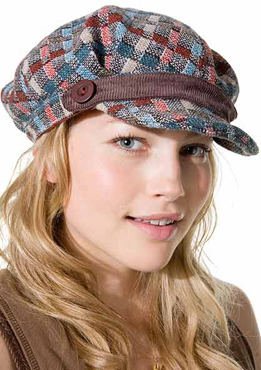
\includegraphics[width=0.5\linewidth]{images/SCP-180-2.jpg}
    \caption*{虽然看上去是美女,但实际上这是一只4龄婆罗洲猩猩。}
\end{figure}

随着寄主的变化SCP-180的外貌也会变化。但是,这种效应仅仅是视觉上的。此物体曾以大礼帽、无沿便帽、棒球帽、扎染印花包头大手帕、发夹、穆斯林妇女佩戴的面纱希贾布、摩托车头盔等形式出现。用核磁共振成像和3D超音波成像显示SCP-180实际上只是一段像是面罩或裹尸布的旧亚麻布或其他布料。将SCP-180正确放在头上实际上会将脸部遮盖起来。研究尚未能解释SCP-180操纵的辐射(可视和红外线)是如何或是为何会产生假象的。
